\documentclass[11pt,]{article}
\usepackage[osf,sc]{mathpazo}
\usepackage{setspace}
\setstretch{1.05}
\usepackage{amssymb,amsmath}
\usepackage{ifxetex,ifluatex}
\usepackage{fixltx2e} % provides \textsubscript
\ifnum 0\ifxetex 1\fi\ifluatex 1\fi=0 % if pdftex
  \usepackage[T1]{fontenc}
  \usepackage[utf8]{inputenc}
\else % if luatex or xelatex
  \ifxetex
    \usepackage{mathspec}
  \else
    \usepackage{fontspec}
  \fi
  \defaultfontfeatures{Ligatures=TeX,Scale=MatchLowercase}
\fi
% use upquote if available, for straight quotes in verbatim environments
\IfFileExists{upquote.sty}{\usepackage{upquote}}{}
% use microtype if available
\IfFileExists{microtype.sty}{%
\usepackage{microtype}
\UseMicrotypeSet[protrusion]{basicmath} % disable protrusion for tt fonts
}{}
\usepackage{hyperref}
\hypersetup{unicode=true,
            pdftitle={Modeling the Effect of U.S. Arms Transfers on FDI},
            pdfauthor={Ben Horvath},
            pdfborder={0 0 0},
            breaklinks=true}
\urlstyle{same}  % don't use monospace font for urls
\usepackage{color}
\usepackage{fancyvrb}
\newcommand{\VerbBar}{|}
\newcommand{\VERB}{\Verb[commandchars=\\\{\}]}
\DefineVerbatimEnvironment{Highlighting}{Verbatim}{commandchars=\\\{\}}
% Add ',fontsize=\small' for more characters per line
\usepackage{framed}
\definecolor{shadecolor}{RGB}{248,248,248}
\newenvironment{Shaded}{\begin{snugshade}}{\end{snugshade}}
\newcommand{\AlertTok}[1]{\textcolor[rgb]{0.94,0.16,0.16}{#1}}
\newcommand{\AnnotationTok}[1]{\textcolor[rgb]{0.56,0.35,0.01}{\textbf{\textit{#1}}}}
\newcommand{\AttributeTok}[1]{\textcolor[rgb]{0.77,0.63,0.00}{#1}}
\newcommand{\BaseNTok}[1]{\textcolor[rgb]{0.00,0.00,0.81}{#1}}
\newcommand{\BuiltInTok}[1]{#1}
\newcommand{\CharTok}[1]{\textcolor[rgb]{0.31,0.60,0.02}{#1}}
\newcommand{\CommentTok}[1]{\textcolor[rgb]{0.56,0.35,0.01}{\textit{#1}}}
\newcommand{\CommentVarTok}[1]{\textcolor[rgb]{0.56,0.35,0.01}{\textbf{\textit{#1}}}}
\newcommand{\ConstantTok}[1]{\textcolor[rgb]{0.00,0.00,0.00}{#1}}
\newcommand{\ControlFlowTok}[1]{\textcolor[rgb]{0.13,0.29,0.53}{\textbf{#1}}}
\newcommand{\DataTypeTok}[1]{\textcolor[rgb]{0.13,0.29,0.53}{#1}}
\newcommand{\DecValTok}[1]{\textcolor[rgb]{0.00,0.00,0.81}{#1}}
\newcommand{\DocumentationTok}[1]{\textcolor[rgb]{0.56,0.35,0.01}{\textbf{\textit{#1}}}}
\newcommand{\ErrorTok}[1]{\textcolor[rgb]{0.64,0.00,0.00}{\textbf{#1}}}
\newcommand{\ExtensionTok}[1]{#1}
\newcommand{\FloatTok}[1]{\textcolor[rgb]{0.00,0.00,0.81}{#1}}
\newcommand{\FunctionTok}[1]{\textcolor[rgb]{0.00,0.00,0.00}{#1}}
\newcommand{\ImportTok}[1]{#1}
\newcommand{\InformationTok}[1]{\textcolor[rgb]{0.56,0.35,0.01}{\textbf{\textit{#1}}}}
\newcommand{\KeywordTok}[1]{\textcolor[rgb]{0.13,0.29,0.53}{\textbf{#1}}}
\newcommand{\NormalTok}[1]{#1}
\newcommand{\OperatorTok}[1]{\textcolor[rgb]{0.81,0.36,0.00}{\textbf{#1}}}
\newcommand{\OtherTok}[1]{\textcolor[rgb]{0.56,0.35,0.01}{#1}}
\newcommand{\PreprocessorTok}[1]{\textcolor[rgb]{0.56,0.35,0.01}{\textit{#1}}}
\newcommand{\RegionMarkerTok}[1]{#1}
\newcommand{\SpecialCharTok}[1]{\textcolor[rgb]{0.00,0.00,0.00}{#1}}
\newcommand{\SpecialStringTok}[1]{\textcolor[rgb]{0.31,0.60,0.02}{#1}}
\newcommand{\StringTok}[1]{\textcolor[rgb]{0.31,0.60,0.02}{#1}}
\newcommand{\VariableTok}[1]{\textcolor[rgb]{0.00,0.00,0.00}{#1}}
\newcommand{\VerbatimStringTok}[1]{\textcolor[rgb]{0.31,0.60,0.02}{#1}}
\newcommand{\WarningTok}[1]{\textcolor[rgb]{0.56,0.35,0.01}{\textbf{\textit{#1}}}}
\usepackage{graphicx,grffile}
\makeatletter
\def\maxwidth{\ifdim\Gin@nat@width>\linewidth\linewidth\else\Gin@nat@width\fi}
\def\maxheight{\ifdim\Gin@nat@height>\textheight\textheight\else\Gin@nat@height\fi}
\makeatother
% Scale images if necessary, so that they will not overflow the page
% margins by default, and it is still possible to overwrite the defaults
% using explicit options in \includegraphics[width, height, ...]{}
\setkeys{Gin}{width=\maxwidth,height=\maxheight,keepaspectratio}
\IfFileExists{parskip.sty}{%
\usepackage{parskip}
}{% else
\setlength{\parindent}{0pt}
\setlength{\parskip}{6pt plus 2pt minus 1pt}
}
\setlength{\emergencystretch}{3em}  % prevent overfull lines
\providecommand{\tightlist}{%
  \setlength{\itemsep}{0pt}\setlength{\parskip}{0pt}}
\setcounter{secnumdepth}{5}
% Redefines (sub)paragraphs to behave more like sections
\ifx\paragraph\undefined\else
\let\oldparagraph\paragraph
\renewcommand{\paragraph}[1]{\oldparagraph{#1}\mbox{}}
\fi
\ifx\subparagraph\undefined\else
\let\oldsubparagraph\subparagraph
\renewcommand{\subparagraph}[1]{\oldsubparagraph{#1}\mbox{}}
\fi

%%% Use protect on footnotes to avoid problems with footnotes in titles
\let\rmarkdownfootnote\footnote%
\def\footnote{\protect\rmarkdownfootnote}

%%% Change title format to be more compact
\usepackage{titling}

% Create subtitle command for use in maketitle
\newcommand{\subtitle}[1]{
  \posttitle{
    \begin{center}\large#1\end{center}
    }
}

\setlength{\droptitle}{-2em}

  \title{Modeling the Effect of U.S. Arms Transfers on FDI}
    \pretitle{\vspace{\droptitle}\centering\huge}
  \posttitle{\par}
    \author{Ben Horvath}
    \preauthor{\centering\large\emph}
  \postauthor{\par}
      \predate{\centering\large\emph}
  \postdate{\par}
    \date{December 9, 2018}

\usepackage{eulervm}

\begin{document}
\maketitle

{
\setcounter{tocdepth}{2}
\tableofcontents
}
Load libraries:

\begin{Shaded}
\begin{Highlighting}[]
\KeywordTok{library}\NormalTok{(corrplot)}
\KeywordTok{library}\NormalTok{(dplyr)}
\KeywordTok{library}\NormalTok{(ggplot2)}
\KeywordTok{library}\NormalTok{(lme4)}

\KeywordTok{source}\NormalTok{(}\StringTok{'../R/multiplot.R'}\NormalTok{)}
\end{Highlighting}
\end{Shaded}

\hypertarget{introduction}{%
\section{Introduction}\label{introduction}}

Corporations and investors can directly invest in enterprises in foreign
countries, as opposed to, for instance, portfolio investments like
stocks and bonds. This type of investment is called \emph{foreign direct
investment}.

Some countries will have specific advantages over others that attract
FDI. Rugman (2001, 157--58) divides them into `harder' and `softer'
advantages. The former are primarily economic---access to natural
resources, a cheaper component of production, etc. Soft locational
advantages refer to intangible benefits, e.g., subjective firm director
preferences.

Political factors must be counted among locational advantages or
disadvantages. When a left-wing government comes to power and threatens
nationalization of large industries, investors are likely to become
wary. International politics advantages have been well-studied. Many
scholars have tested and confirmed the hypothesis that `alliances have a
direct, statistically significant, and large effect on bilateral trade'
(Gowa 1994, 54; see also Gowa and Mansfield 1993 and Long 2003). Other
scholars have examined FDI in this context. Biglaiser and DeRouen (2007)
and Little and Leblong (2004) found that the presence of U.S. troops in
a potential host country increases the level of incoming FDI, i.e., is a
locational advantage to investors.

This analysis provides another test of the relationship between FDI and
international security arrangements: Are U.S. arms transfers, like the
presence of the U.S. military itself, a locational advantage to
investors? There are a number of major reasons to believe this might be
so. First, military aid suggests a friendly atmosphere between the U.S.
and potential host. Second, corporate interests often correspond to the
interests of the U.S. government: To quote Gilpin, ``although the
interests of American corporations and U.S. foreign policy objectives
have collided on many occasions, a complementarity of interests has
tended to exist between the corporations and the U.S. government''
(1987, 241). Third, like the presence of U.S. soldiers, military aid can
(but does not always) signal stability to investors and a decreased
chance of political or econmomic disruption.

To test this theory, I assemble a data set of FDI flows from the U.S.,
military sales from the U.S., and supplementary variables likely to also
affect FDI flows. I run numerous kinds of regressions, in search of the
best model of this phenomenon.

\hypertarget{data-collection}{%
\section{Data Collection}\label{data-collection}}

I assemble a dataset with the following variables. For full citations,
see the references at the end of the paper.

\begin{itemize}
\item
  \textbf{FDI}. The OECD provides FDI data for U.S. outflows on its
  website, from 2003 to 2013. These years will have to bound this study
  temporally:
  \url{https://stats.oecd.org/index.aspx?DataSetCode=FDI_FLOW_PARTNER}
\item
  \textbf{Arms Transfers}. The Stockholm International Peace Research
  Institute maintains a database of arms transfers:
  \url{https://www.sipri.org/databases/armstransfers}. The value has
  been `normalized' by the researchers themselves to account for
  fluctuations in the market value of weapons as well as allowing
  comparability between, e.g., 100 assault rifles and 2 large
  artilleries.
\item
  \textbf{Yearly Population}. This is available for most countries on a
  yearly basis via the UN:
  \url{https://population.un.org/wpp/Download/Standard/Population/}.
\item
  \textbf{Presence of Conflict}. Political scientists testing hypotheses
  on armed conflict frequently make use of the Armed Conflict dataset,
  available at: \url{http://ucdp.uu.se/downloads/\#d3}. This dataset is
  very detailed in describing exactly the kind of conflict. Instead, I
  will use a dichotomous variable: 0 for no conflict, 1 for conflict.
\item
  \textbf{Regime Type}. This is available in one of the most popular
  political science datasets, the Polity dataset. It encodes regime type
  in a range from perfectly democratic to perfectly autocratic for most
  countries from 1800 on. Specifically I will use the Polity2 variable:
  \url{http://www.systemicpeace.org/inscrdata.html}. See also the user
  manual: \url{http://www.systemicpeace.org/inscr/p4manualv2017.pdf}.
  Although Polity2 is a scale from -10 to 10, it is often coded to an
  ordinal variable with the following levels: autocracy, closed
  anocracy, open anocracy, democracy, full democracy, and
  conflict/occupied.
\item
  \textbf{Alliances}. The Correlates of War project maintains another
  popular data set encoding international alliances in `dyadic' form a
  year-to-year basis:
  \url{http://www.correlatesofwar.org/data-sets/formal-alliances}.
\item
  \textbf{Distance}. Kristian Gleditsch developed a data set containing
  the distance between capital cities, which we'll use to proxy
  distance: \url{http://ksgleditsch.com/data-5.html}, using this system
  of country codes: \url{http://ksgleditsch.com/statelist.html}.
\item
  \textbf{GDP}. Where else but the World Bank?:
  \url{https://data.worldbank.org/indicator/NY.GDP.MKTP.CD}
\end{itemize}

Assembling the complete dataset is a lengthy affair. I have contained it
to the \texttt{R/clean\_data.R} script.

I will simply load the finished dataset here:

\begin{Shaded}
\begin{Highlighting}[]
\NormalTok{df <-}\StringTok{ }\KeywordTok{read.csv}\NormalTok{(}\StringTok{'../data/clean/master_dataset.tsv'}\NormalTok{, }\DataTypeTok{sep=}\StringTok{'}\CharTok{\textbackslash{}t}\StringTok{'}\NormalTok{, }
               \DataTypeTok{stringsAsFactors=}\OtherTok{FALSE}\NormalTok{)}
\end{Highlighting}
\end{Shaded}

The primary barrier to assembling this data set was standardization of
country names. For instance, in some data sets, the Vatican is called
`Holy See (Vatican City State),' and others, simply `Holy See.' There
are also occasional typos, e.g., `NewZealand' or `SriLanka' rather than
`New Zealand' or `Sri Lanka.' Countries with accented characters posed
another issue.

Tediously and laborously, I standardized each seperate piece of the
dataset by hand.

There is one more wrinkle to deal with. Since we are testing a theory
about how agents react to information, our dataset has to reflect that
agent's knowledge. To do so, each of the independent variables is lagged
by one year. Thus, for instance, the model will be trained on data from
2003 to predict a country's \texttt{fdi} in 2004:

\begin{Shaded}
\begin{Highlighting}[]
\NormalTok{df <-}\StringTok{ }\NormalTok{df }\OperatorTok
\StringTok{    }\KeywordTok{group_by}\NormalTok{(country) }\OperatorTok
\StringTok{    }\KeywordTok{mutate}\NormalTok{(}\DataTypeTok{population=}\KeywordTok{lag}\NormalTok{(population, }\DataTypeTok{order_by=}\NormalTok{year),}
           \DataTypeTok{arms_exports=}\KeywordTok{lag}\NormalTok{(arms_exports, }\DataTypeTok{order_by=}\NormalTok{year),}
           \DataTypeTok{conflict=}\KeywordTok{lag}\NormalTok{(conflict, }\DataTypeTok{order_by=}\NormalTok{year),}
           \DataTypeTok{alliance=}\KeywordTok{lag}\NormalTok{(alliance, }\DataTypeTok{order_by=}\NormalTok{year),}
           \DataTypeTok{gdp=}\KeywordTok{lag}\NormalTok{(gdp, }\DataTypeTok{order_by=}\NormalTok{year),}
           \DataTypeTok{gdp_perc_growth=}\KeywordTok{lag}\NormalTok{(gdp_perc_growth, }\DataTypeTok{order_by=}\NormalTok{year),}
           \DataTypeTok{regime_type=}\KeywordTok{lag}\NormalTok{(regime_type, }\DataTypeTok{order_by=}\NormalTok{year)) }\OperatorTok
\StringTok{    }\KeywordTok{na.omit}\NormalTok{()}
\end{Highlighting}
\end{Shaded}

The accurately evaluate each of the models, I partition the data into a
train (70 percent) and test set, where the last three years of the
dataset for each country are loaded into the test set (approximately 30
percent of the observations). This will provide a good measure of how
well the developed models can be expected to perform in reality.

\begin{Shaded}
\begin{Highlighting}[]
\NormalTok{train <-}\StringTok{ }\NormalTok{df }\OperatorTok\StringTok{ }\KeywordTok{filter}\NormalTok{(year }\OperatorTok{<=}\StringTok{ }\DecValTok{2010}\NormalTok{)}

\NormalTok{test <-}\StringTok{ }\NormalTok{df }\OperatorTok\StringTok{ }\KeywordTok{filter}\NormalTok{(year }\OperatorTok{>}\StringTok{ }\DecValTok{2010}\NormalTok{)}

\KeywordTok{write.table}\NormalTok{(train, }\StringTok{'../data/clean/train.tsv'}\NormalTok{, }\DataTypeTok{sep=}\StringTok{'}\CharTok{\textbackslash{}t}\StringTok{'}\NormalTok{, }
            \DataTypeTok{row.names=}\OtherTok{FALSE}\NormalTok{)}
\KeywordTok{write.table}\NormalTok{(test, }\StringTok{'../data/clean/test.tsv'}\NormalTok{, }\DataTypeTok{sep=}\StringTok{'}\CharTok{\textbackslash{}t}\StringTok{'}\NormalTok{, }
            \DataTypeTok{row.names=}\OtherTok{FALSE}\NormalTok{)}

\CommentTok{# remove from workspace for now to keep models uncontaminated}
\KeywordTok{rm}\NormalTok{(test)}
\end{Highlighting}
\end{Shaded}

\hypertarget{exploratory-data-analysis}{%
\section{Exploratory Data Analysis}\label{exploratory-data-analysis}}

The training set:

\begin{Shaded}
\begin{Highlighting}[]
\KeywordTok{head}\NormalTok{(train)}
\end{Highlighting}
\end{Shaded}

\begin{verbatim}
## # A tibble: 6 x 11
## # Groups:   country [1]
##    year country      fdi population arms_exports conflict alliance km_dist
##   <int> <chr>      <dbl>      <int>        <int>    <int>    <int>   <int>
## 1  2005 Afghani~  0.       24118979            0        1        0   11132
## 2  2006 Afghani~  0.       25070798           19        1        0   11132
## 3  2007 Afghani~  0.       25893450            0        1        0   11132
## 4  2008 Afghani~  0.       26616792           22        1        0   11132
## 5  2009 Afghani~ -1.00e6   27294031           78        1        0   11132
## 6  2010 Afghani~ -1.00e6   28004331          280        1        0   11132
## # ... with 3 more variables: gdp <dbl>, gdp_perc_growth <dbl>,
## #   regime_type <chr>
\end{verbatim}

To get a sense of the range of our dependent variable and main
independent variable:

\begin{Shaded}
\begin{Highlighting}[]
\KeywordTok{mean}\NormalTok{(train}\OperatorTok{$}\NormalTok{fdi)}
\end{Highlighting}
\end{Shaded}

\begin{verbatim}
## [1] 1488869736
\end{verbatim}

Mean \texttt{fdi} is about \$1.5 billion, while median is only \$1
million. This suggests a \emph{highly} right-skewed distribution:

\begin{Shaded}
\begin{Highlighting}[]
\KeywordTok{quantile}\NormalTok{(train}\OperatorTok{$}\NormalTok{fdi, }\KeywordTok{c}\NormalTok{(}\DecValTok{0}\NormalTok{, }\FloatTok{.25}\NormalTok{, }\FloatTok{0.5}\NormalTok{, }\FloatTok{0.75}\NormalTok{, }\FloatTok{0.9}\NormalTok{, }\FloatTok{0.95}\NormalTok{, }\FloatTok{0.99}\NormalTok{))}
\end{Highlighting}
\end{Shaded}

\begin{verbatim}
##          0%         25%         50%         75%         90%         95% 
## -1.9284e+10  0.0000e+00  1.0000e+06  4.4700e+08  3.0580e+09  8.5720e+09 
##         99% 
##  3.0351e+10
\end{verbatim}

The min of \texttt{fdi} is -\$20 billion. Negative FDI seems puzzling.
According to this World Bank explainer
\url{https://www.oecd.org/daf/inv/FDI-statistics-explanatory-notes.pdf},

\begin{quote}
FDI financial transactions may be negative for three reasons. First, if
there is disinvestment in assets--- that is, the direct investor sells
its interest in a direct investment enterprise to a third party or back
to the direct investment enterprise. Second, if the parent borrowed
money from its affiliate or if the affiliate paid off a loan from its
direct investor. Third, if reinvested earnings are negative. Reinvested
earnings are negative if the affiliate loses money or if the dividends
paid out to the direct investor are greater than the income recorded in
that period. Negative FDI positions largely result when the loans from
the affiliate to its parent exceed the loans and equity capital given by
the parent to the affiliate. This is most likely to occur when FDI
statistics are presented by partner country.
\end{quote}

W see that middle 50 percent of the variable is between \$0 and about
\$150 million, and the top one percent is greater than \$30 billion.

\texttt{arms\_exports} is less extreme, but still skewed,

\begin{Shaded}
\begin{Highlighting}[]
\KeywordTok{mean}\NormalTok{(train}\OperatorTok{$}\NormalTok{arms_exports)}
\end{Highlighting}
\end{Shaded}

\begin{verbatim}
## [1] 44.59256
\end{verbatim}

\begin{Shaded}
\begin{Highlighting}[]
\KeywordTok{quantile}\NormalTok{(train}\OperatorTok{$}\NormalTok{arms_exports, }\KeywordTok{c}\NormalTok{(}\DecValTok{0}\NormalTok{, }\FloatTok{.25}\NormalTok{, }\FloatTok{0.5}\NormalTok{, }\FloatTok{0.75}\NormalTok{, }\FloatTok{0.9}\NormalTok{, }\FloatTok{0.95}\NormalTok{, }\FloatTok{0.99}\NormalTok{))}
\end{Highlighting}
\end{Shaded}

\begin{verbatim}
##    0%   25%   50%   75%   90%   95%   99% 
##   0.0   0.0   0.0   5.0  89.0 303.0 847.8
\end{verbatim}

with a mean of 44.5 arms units and a median of 0. The 25th and 75th
percentile ranges from 0 to 5. The largest arms transfers seem to make
up about 5 percent of the total data set.

\hypertarget{distributions}{%
\subsection{Distributions}\label{distributions}}

For the first pass through, let's examine the distributions of the
numeric variables:

\begin{Shaded}
\begin{Highlighting}[]
\NormalTok{hist_fdi <-}\StringTok{ }\KeywordTok{ggplot}\NormalTok{(train, }\KeywordTok{aes}\NormalTok{(}\DataTypeTok{x=}\NormalTok{fdi)) }\OperatorTok{+}\StringTok{ }
\StringTok{    }\KeywordTok{geom_histogram}\NormalTok{(}\DataTypeTok{colour=}\StringTok{"black"}\NormalTok{, }\DataTypeTok{fill=}\StringTok{"white"}\NormalTok{)}

\NormalTok{hist_arms <-}\StringTok{ }\KeywordTok{ggplot}\NormalTok{(train, }\KeywordTok{aes}\NormalTok{(}\DataTypeTok{x=}\NormalTok{arms_exports)) }\OperatorTok{+}\StringTok{ }
\StringTok{    }\KeywordTok{geom_histogram}\NormalTok{(}\DataTypeTok{colour=}\StringTok{"black"}\NormalTok{, }\DataTypeTok{fill=}\StringTok{"white"}\NormalTok{)}

\NormalTok{hist_pop <-}\StringTok{ }\KeywordTok{ggplot}\NormalTok{(train, }\KeywordTok{aes}\NormalTok{(}\DataTypeTok{x=}\NormalTok{population)) }\OperatorTok{+}\StringTok{ }
\StringTok{    }\KeywordTok{geom_histogram}\NormalTok{(}\DataTypeTok{colour=}\StringTok{"black"}\NormalTok{, }\DataTypeTok{fill=}\StringTok{"white"}\NormalTok{)}

\NormalTok{hist_conflict <-}\StringTok{ }\KeywordTok{ggplot}\NormalTok{(train, }\KeywordTok{aes}\NormalTok{(}\DataTypeTok{x=}\NormalTok{conflict)) }\OperatorTok{+}\StringTok{ }
\StringTok{    }\KeywordTok{geom_histogram}\NormalTok{(}\DataTypeTok{colour=}\StringTok{"black"}\NormalTok{, }\DataTypeTok{fill=}\StringTok{"white"}\NormalTok{)}

\NormalTok{hist_alliance <-}\StringTok{ }\KeywordTok{ggplot}\NormalTok{(train, }\KeywordTok{aes}\NormalTok{(}\DataTypeTok{x=}\NormalTok{alliance)) }\OperatorTok{+}\StringTok{ }
\StringTok{    }\KeywordTok{geom_histogram}\NormalTok{(}\DataTypeTok{colour=}\StringTok{"black"}\NormalTok{, }\DataTypeTok{fill=}\StringTok{"white"}\NormalTok{)}

\NormalTok{hist_dist <-}\StringTok{ }\KeywordTok{ggplot}\NormalTok{(train, }\KeywordTok{aes}\NormalTok{(}\DataTypeTok{x=}\NormalTok{km_dist)) }\OperatorTok{+}\StringTok{ }
\StringTok{    }\KeywordTok{geom_histogram}\NormalTok{(}\DataTypeTok{colour=}\StringTok{"black"}\NormalTok{, }\DataTypeTok{fill=}\StringTok{"white"}\NormalTok{)}

\NormalTok{hist_gdp <-}\StringTok{ }\KeywordTok{ggplot}\NormalTok{(train, }\KeywordTok{aes}\NormalTok{(}\DataTypeTok{x=}\NormalTok{gdp)) }\OperatorTok{+}\StringTok{ }
\StringTok{    }\KeywordTok{geom_histogram}\NormalTok{(}\DataTypeTok{colour=}\StringTok{"black"}\NormalTok{, }\DataTypeTok{fill=}\StringTok{"white"}\NormalTok{)}

\NormalTok{hist_growth <-}\StringTok{ }\KeywordTok{ggplot}\NormalTok{(train, }\KeywordTok{aes}\NormalTok{(}\DataTypeTok{x=}\NormalTok{gdp_perc_growth)) }\OperatorTok{+}\StringTok{ }
\StringTok{    }\KeywordTok{geom_histogram}\NormalTok{(}\DataTypeTok{colour=}\StringTok{"black"}\NormalTok{, }\DataTypeTok{fill=}\StringTok{"white"}\NormalTok{)}

\KeywordTok{multiplot}\NormalTok{(hist_fdi, hist_arms, hist_pop, hist_conflict, }
\NormalTok{          hist_alliance, hist_dist, hist_gdp, hist_growth, }\DataTypeTok{cols=}\DecValTok{2}\NormalTok{)}
\end{Highlighting}
\end{Shaded}

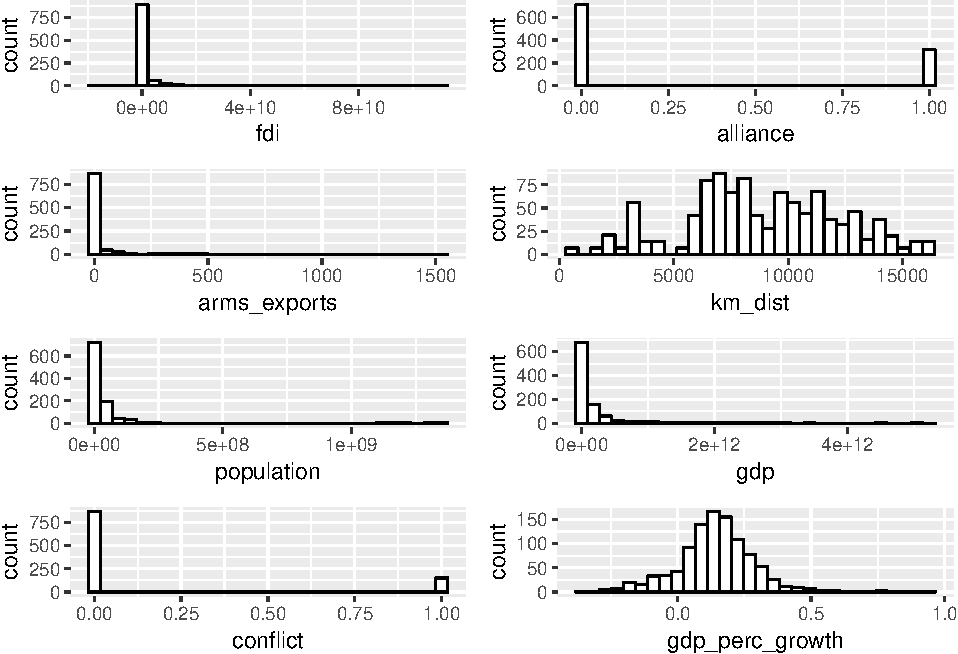
\includegraphics{report_files/figure-latex/unnamed-chunk-9-1.pdf}

From these graphs it's clear there are only two `nice' variables:
\texttt{km\_dist} and \texttt{gdp\_perc\_growth}, i.e., the only ones
approximately normally distributed.

Our two most important variables, \texttt{fdi} and
\texttt{arms\_exports} are not normal. They are both
\emph{zero-inflated}, with a long right tail. This may prove challenging
in attempting to model them with standard linear regression models.

The variables \texttt{gdp} and \texttt{population} also have a small
central tendancy, with a long right tail. This reflects the facts that
most countries have a small population with a correspondingly small GDP,
and that there are a few large countries with large GDPs.

The remaining variables are dichotomous, \texttt{conflict} and
\texttt{alliance}. These plots show that of the observations in the
dataset are in a time of peace, and that most of them did not occur when
the country was allied with the United States.

\hypertarget{associations-and-correlations}{%
\subsection{Associations and
Correlations}\label{associations-and-correlations}}

The next step is to take a look for associations in our data set:

\begin{Shaded}
\begin{Highlighting}[]
\NormalTok{scat_arms <-}\StringTok{ }\KeywordTok{ggplot}\NormalTok{(train, }\KeywordTok{aes}\NormalTok{(}\DataTypeTok{x=}\NormalTok{arms_exports, }\DataTypeTok{y=}\NormalTok{fdi)) }\OperatorTok{+}
\StringTok{    }\KeywordTok{geom_point}\NormalTok{() }\OperatorTok{+}
\StringTok{    }\KeywordTok{geom_smooth}\NormalTok{()}

\NormalTok{scat_pop <-}\StringTok{ }\KeywordTok{ggplot}\NormalTok{(train, }\KeywordTok{aes}\NormalTok{(}\DataTypeTok{x=}\NormalTok{population, }\DataTypeTok{y=}\NormalTok{fdi)) }\OperatorTok{+}
\StringTok{    }\KeywordTok{geom_point}\NormalTok{() }\OperatorTok{+}
\StringTok{    }\KeywordTok{geom_smooth}\NormalTok{()}

\NormalTok{scat_conflict <-}\StringTok{ }\KeywordTok{ggplot}\NormalTok{(train, }\KeywordTok{aes}\NormalTok{(}\DataTypeTok{x=}\NormalTok{conflict, }\DataTypeTok{y=}\NormalTok{fdi)) }\OperatorTok{+}
\StringTok{    }\KeywordTok{geom_point}\NormalTok{() }\OperatorTok{+}
\StringTok{    }\KeywordTok{geom_smooth}\NormalTok{()}

\NormalTok{scat_alliance <-}\StringTok{ }\KeywordTok{ggplot}\NormalTok{(train, }\KeywordTok{aes}\NormalTok{(}\DataTypeTok{x=}\NormalTok{alliance, }\DataTypeTok{y=}\NormalTok{fdi)) }\OperatorTok{+}
\StringTok{    }\KeywordTok{geom_point}\NormalTok{() }\OperatorTok{+}
\StringTok{    }\KeywordTok{geom_smooth}\NormalTok{()}

\NormalTok{scat_dist <-}\StringTok{ }\KeywordTok{ggplot}\NormalTok{(train, }\KeywordTok{aes}\NormalTok{(}\DataTypeTok{x=}\NormalTok{km_dist, }\DataTypeTok{y=}\NormalTok{fdi)) }\OperatorTok{+}
\StringTok{    }\KeywordTok{geom_point}\NormalTok{() }\OperatorTok{+}
\StringTok{    }\KeywordTok{geom_smooth}\NormalTok{()}

\NormalTok{scat_gdp <-}\StringTok{ }\KeywordTok{ggplot}\NormalTok{(train, }\KeywordTok{aes}\NormalTok{(}\DataTypeTok{x=}\NormalTok{gdp, }\DataTypeTok{y=}\NormalTok{fdi)) }\OperatorTok{+}
\StringTok{    }\KeywordTok{geom_point}\NormalTok{() }\OperatorTok{+}
\StringTok{    }\KeywordTok{geom_smooth}\NormalTok{()}

\NormalTok{scat_growth <-}\StringTok{ }\KeywordTok{ggplot}\NormalTok{(train, }\KeywordTok{aes}\NormalTok{(}\DataTypeTok{x=}\NormalTok{gdp_perc_growth, }\DataTypeTok{y=}\NormalTok{fdi)) }\OperatorTok{+}
\StringTok{    }\KeywordTok{geom_point}\NormalTok{() }\OperatorTok{+}
\StringTok{    }\KeywordTok{geom_smooth}\NormalTok{()}

\KeywordTok{multiplot}\NormalTok{(scat_arms, scat_pop, scat_conflict, scat_alliance,}
\NormalTok{          scat_dist, scat_gdp, scat_growth, }\DataTypeTok{cols=}\DecValTok{2}\NormalTok{)}
\end{Highlighting}
\end{Shaded}

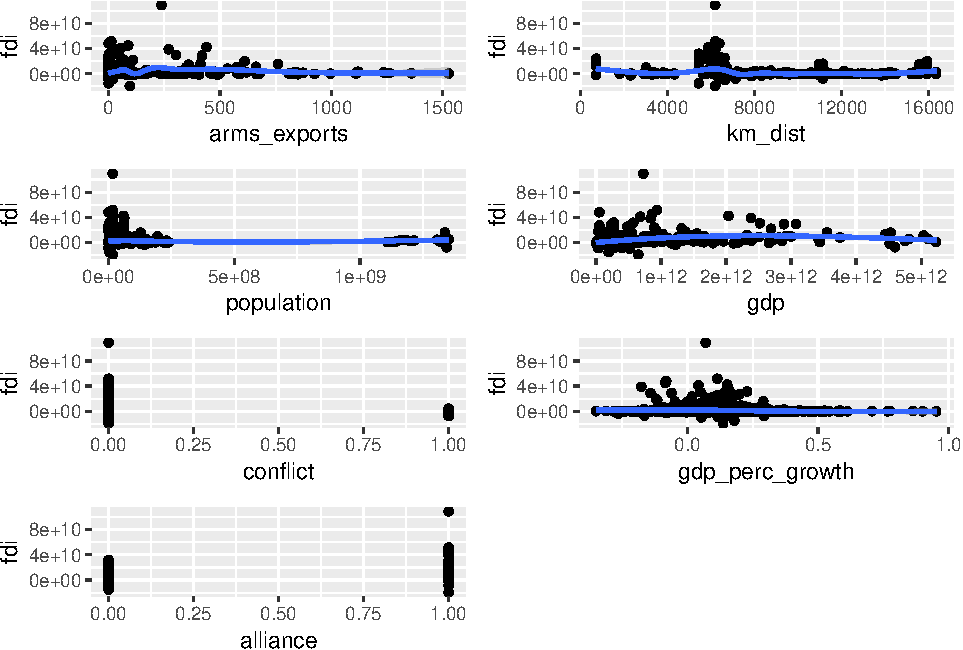
\includegraphics{report_files/figure-latex/unnamed-chunk-10-1.pdf}

Few of these variables are related to \texttt{fdi} in a
straight-forward, linear way.

Examining our categorical variable, \texttt{regime\_type}:

\begin{Shaded}
\begin{Highlighting}[]
\KeywordTok{ggplot}\NormalTok{(train, }\KeywordTok{aes}\NormalTok{(}\DataTypeTok{x=}\NormalTok{regime_type, }\DataTypeTok{y=}\NormalTok{fdi)) }\OperatorTok{+}
\StringTok{    }\KeywordTok{geom_boxplot}\NormalTok{()}
\end{Highlighting}
\end{Shaded}

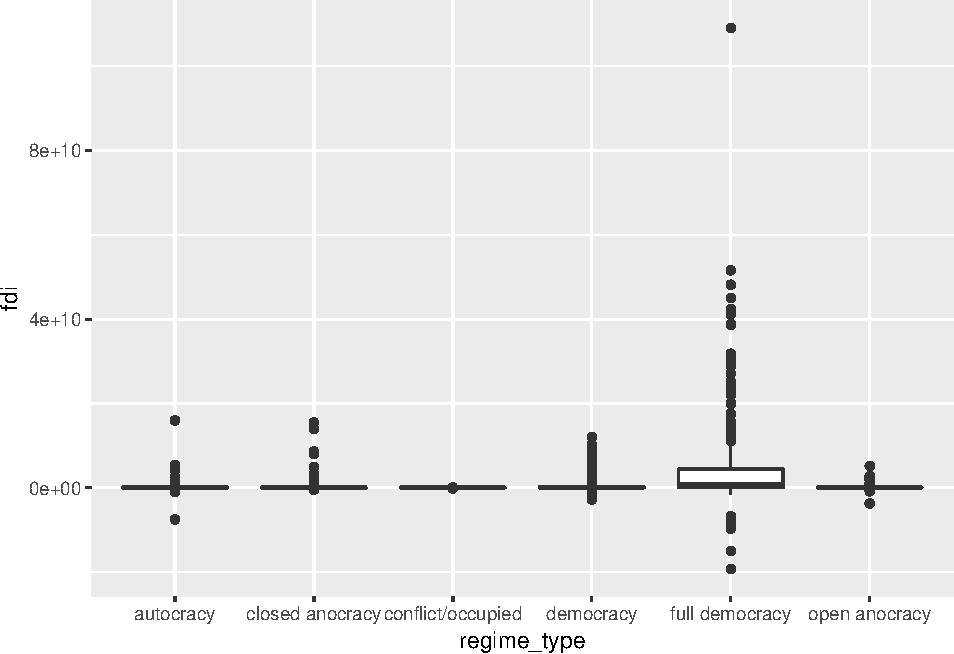
\includegraphics{report_files/figure-latex/unnamed-chunk-11-1.pdf}

Full democracies obviously receive the most FDI from the U.S., though
autocratic countries still receive some. Conflicted/occupied countries
recieve very little, which makes sense.

The correlation matrix of the numerical variables:

\begin{Shaded}
\begin{Highlighting}[]
\NormalTok{train_cor <-}\StringTok{ }\KeywordTok{cor}\NormalTok{(train[, }\KeywordTok{c}\NormalTok{(}\DecValTok{3}\OperatorTok{:}\DecValTok{10}\NormalTok{)])}
\KeywordTok{corrplot}\NormalTok{(train_cor, }\DataTypeTok{type=}\StringTok{'lower'}\NormalTok{, }\DataTypeTok{method=}\StringTok{'number'}\NormalTok{)}
\end{Highlighting}
\end{Shaded}

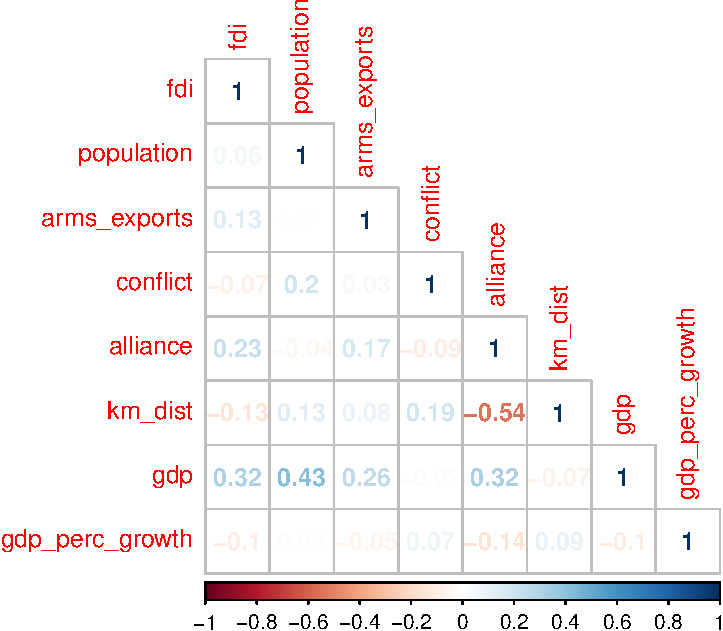
\includegraphics{report_files/figure-latex/unnamed-chunk-12-1.pdf}

Unfortunately for us, the correlation between the main variables of
interest, \texttt{fdi} and \texttt{arms\_exports} is low, only 0.13.
But, more hopefully, few of our other independent variables are
correlated, which protects our regression models from multicollinearity.

The two worrying relationships are \texttt{gdp} and \texttt{population},
which are naturally related, with a correlation of 0.43. More
interesting is the correlation of \texttt{km\_dist} and
\texttt{alliance} (-0.54). This suggests that the further away a country
is from the U.S., the less likely an alliance with it will be. This is a
non-intuitive finding, but could possibly be explained by the difficulty
of projecting force across large distances and oceans.

\hypertarget{statistical-analysis}{%
\section{Statistical Analysis}\label{statistical-analysis}}

\hypertarget{inferential-statistics}{%
\subsection{Inferential Statistics}\label{inferential-statistics}}

We've seen above that appears to be some kind of association between
\texttt{regime\_type} and \texttt{fdi}, where democracies recieve more
trade that autocracies. This section will formally test this, with the
hypotheses,

\begin{quote}
\(H_0\): \(\mu_{democracy} - \mu_{autocracy} = 0\)
\end{quote}

\begin{quote}
\(H_1\): \(\mu_{democracy} - \mu_{autocracy} > 0\)
\end{quote}

I create two vectors of \texttt{fdi}, one for country-years where the
country was either a `full democracy' or a `democracy,' and the other
for countries that are an `autocracy' or `closed anonocracy'. Their
respective distributions are plotted:

\begin{Shaded}
\begin{Highlighting}[]
\NormalTok{x_demo <-}\StringTok{ }\NormalTok{train }\OperatorTok
\StringTok{    }\KeywordTok{filter}\NormalTok{(regime_type }\OperatorTok{==}\StringTok{ 'full democracy'} \OperatorTok{|}\StringTok{ }\NormalTok{regime_type }\OperatorTok{==}\StringTok{ 'democracy'}\NormalTok{) }\OperatorTok\StringTok{ }
\StringTok{    }\KeywordTok{select}\NormalTok{(fdi)}

\NormalTok{x_auto <-}\StringTok{ }\NormalTok{train }\OperatorTok
\StringTok{    }\KeywordTok{filter}\NormalTok{(regime_type }\OperatorTok{==}\StringTok{ 'autocracy'} \OperatorTok{|}\StringTok{ }\NormalTok{regime_type }\OperatorTok{==}\StringTok{ 'closed anocracy'}\NormalTok{) }\OperatorTok
\StringTok{    }\KeywordTok{select}\NormalTok{(fdi)}
    
\NormalTok{hist_demo <-}\StringTok{ }\KeywordTok{ggplot}\NormalTok{(x_demo, }\KeywordTok{aes}\NormalTok{(}\DataTypeTok{x=}\NormalTok{fdi)) }\OperatorTok{+}
\StringTok{    }\KeywordTok{geom_histogram}\NormalTok{(}\DataTypeTok{colour=}\StringTok{"black"}\NormalTok{, }\DataTypeTok{fill=}\StringTok{"white"}\NormalTok{)}
\NormalTok{hist_auto <-}\StringTok{ }\KeywordTok{ggplot}\NormalTok{(x_auto, }\KeywordTok{aes}\NormalTok{(}\DataTypeTok{x=}\NormalTok{fdi)) }\OperatorTok{+}
\StringTok{    }\KeywordTok{geom_histogram}\NormalTok{(}\DataTypeTok{colour=}\StringTok{"black"}\NormalTok{, }\DataTypeTok{fill=}\StringTok{"white"}\NormalTok{)}

\KeywordTok{multiplot}\NormalTok{(hist_demo, hist_auto, }\DataTypeTok{cols=}\DecValTok{2}\NormalTok{)}
\end{Highlighting}
\end{Shaded}

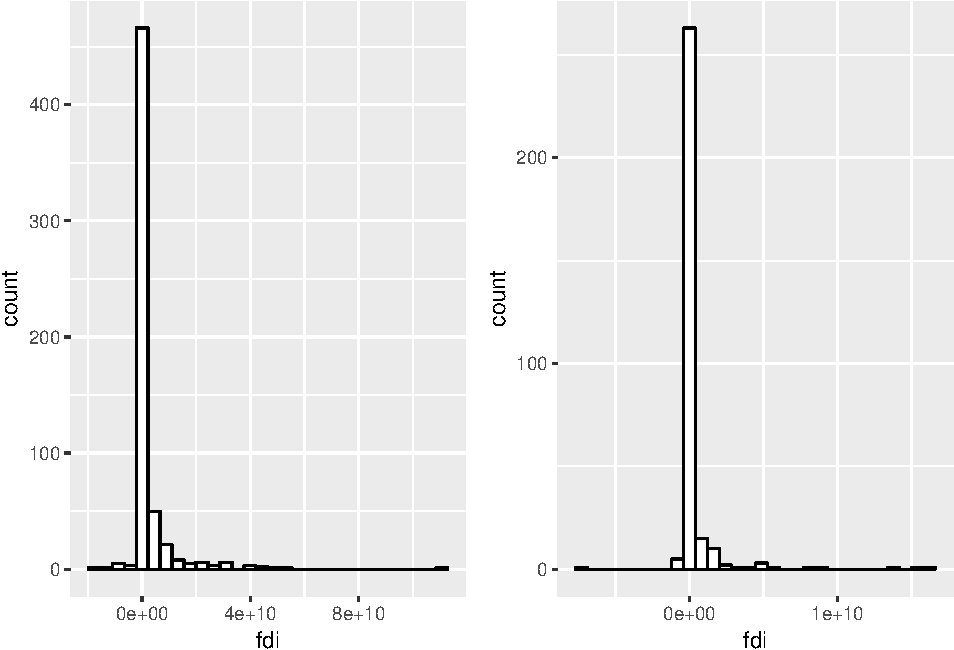
\includegraphics{report_files/figure-latex/unnamed-chunk-13-1.pdf}

The distributions suggest a couple of problems with this hypothesis
test: Because of the skew and the excessive zeros, neither of these
aappear close to a normal distribution. Additionally, the variance of
the two samples are quite different. I will carry on the hypothesis
test, with the hopes that the larger sample size and R's
\texttt{var.equal=FALSE} setting will carry me through:

\begin{Shaded}
\begin{Highlighting}[]
\KeywordTok{t.test}\NormalTok{(x_demo}\OperatorTok{$}\NormalTok{fdi, x_auto}\OperatorTok{$}\NormalTok{fdi, }\DataTypeTok{alternative =} \StringTok{'greater'}\NormalTok{, }
       \DataTypeTok{var.equal =} \OtherTok{FALSE}\NormalTok{, }\DataTypeTok{conf.level =} \FloatTok{0.95}\NormalTok{)}
\end{Highlighting}
\end{Shaded}

\begin{verbatim}
## 
##  Welch Two Sample t-test
## 
## data:  x_demo$fdi and x_auto$fdi
## t = 5.6175, df = 686.26, p-value = 1.409e-08
## alternative hypothesis: true difference in means is greater than 0
## 95 percent confidence interval:
##  1407487063        Inf
## sample estimates:
##  mean of x  mean of y 
## 2365246998  373876221
\end{verbatim}

This \(t\)-test suggetss we should reject the null hypothesis \(H_0\)
that the mean \texttt{fdi} is the same for both democracies and
autocracies. This result is very significant, with a \(t\)-value of
5.62! The larger sample size, the obvious difference between the two
means, and the high significance allay most of my concerns about the
violations noted above.

\hypertarget{models}{%
\subsection{Models}\label{models}}

Each model will be evaluated by its performance on the test set. The
metric to optimize is means squared errors (MSE):

\begin{Shaded}
\begin{Highlighting}[]
\NormalTok{mse <-}\StringTok{ }\ControlFlowTok{function}\NormalTok{(m) }\KeywordTok{mean}\NormalTok{(}\KeywordTok{resid}\NormalTok{(m)}\OperatorTok{^}\DecValTok{2}\NormalTok{)}

\NormalTok{calc_r2 <-}\StringTok{ }\ControlFlowTok{function}\NormalTok{(y, y_hat) \{}
\NormalTok{    rss <-}\StringTok{ }\KeywordTok{sum}\NormalTok{((y_hat }\OperatorTok{-}\StringTok{ }\NormalTok{y)}\OperatorTok{^}\DecValTok{2}\NormalTok{)}
\NormalTok{    tss <-}\StringTok{ }\KeywordTok{sum}\NormalTok{((y }\OperatorTok{-}\StringTok{ }\KeywordTok{mean}\NormalTok{(y_hat))}\OperatorTok{^}\DecValTok{2}\NormalTok{)}
    \KeywordTok{return}\NormalTok{(}\DecValTok{1} \OperatorTok{-}\StringTok{ }\NormalTok{(rss}\OperatorTok{/}\NormalTok{tss))}
\NormalTok{\}}
\end{Highlighting}
\end{Shaded}

Attention will be paid to \(R^2\) as well as performance on training
set. However, \(MSE\) on the test set is the ultimate metric to
minimize.

\hypertarget{m_0-predicting-the-mean}{%
\subsubsection{\texorpdfstring{\(M_0\): Predicting the
Mean}{M\_0: Predicting the Mean}}\label{m_0-predicting-the-mean}}

For the purposes of establishing a baseline performance, the first model
will be a dummy model, predicting only the average FDI.

\begin{Shaded}
\begin{Highlighting}[]
\NormalTok{m0 <-}\StringTok{ }\KeywordTok{lm}\NormalTok{(fdi }\OperatorTok{~}\StringTok{ }\DecValTok{1}\NormalTok{, train)}
\KeywordTok{mse}\NormalTok{(m0)}
\end{Highlighting}
\end{Shaded}

\begin{verbatim}
## [1] 4.024362e+19
\end{verbatim}

With an MSE of over \(4e^{19}\) (dollars), this model performs very
poorly. Hopefully further iteration can improve it.

\hypertarget{m_1-linear-model-all-variables}{%
\subsubsection{\texorpdfstring{\(M_1\): Linear Model, All
Variables}{M\_1: Linear Model, All Variables}}\label{m_1-linear-model-all-variables}}

\begin{Shaded}
\begin{Highlighting}[]
\NormalTok{m1 <-}\StringTok{ }\KeywordTok{lm}\NormalTok{(fdi }\OperatorTok{~}\StringTok{ }\NormalTok{population }\OperatorTok{+}\StringTok{ }\NormalTok{arms_exports }\OperatorTok{+}\StringTok{ }\KeywordTok{as.factor}\NormalTok{(conflict) }\OperatorTok{+}\StringTok{ }
\StringTok{               }\KeywordTok{as.factor}\NormalTok{(alliance) }\OperatorTok{+}\StringTok{ }\NormalTok{km_dist }\OperatorTok{+}\StringTok{ }\NormalTok{gdp }\OperatorTok{+}\StringTok{ }\NormalTok{gdp_perc_growth }\OperatorTok{+}
\StringTok{               }\KeywordTok{as.factor}\NormalTok{(regime_type), train)}
\KeywordTok{summary}\NormalTok{(m1)}
\end{Highlighting}
\end{Shaded}

\begin{verbatim}
## 
## Call:
## lm(formula = fdi ~ population + arms_exports + as.factor(conflict) + 
##     as.factor(alliance) + km_dist + gdp + gdp_perc_growth + as.factor(regime_type), 
##     data = train)
## 
## Residuals:
##        Min         1Q     Median         3Q        Max 
## -2.502e+10 -1.125e+09 -1.353e+08  3.409e+08  1.029e+11 
## 
## Coefficients:
##                                           Estimate Std. Error t value
## (Intercept)                              9.639e+08  8.463e+08   1.139
## population                              -4.508e-01  1.483e+00  -0.304
## arms_exports                             1.802e+06  1.260e+06   1.429
## as.factor(conflict)1                    -2.019e+08  5.622e+08  -0.359
## as.factor(alliance)1                     7.686e+08  5.530e+08   1.390
## km_dist                                 -8.739e+04  6.836e+04  -1.278
## gdp                                      2.123e-03  3.586e-04   5.922
## gdp_perc_growth                         -1.321e+09  1.266e+09  -1.044
## as.factor(regime_type)closed anocracy    4.451e+08  6.798e+08   0.655
## as.factor(regime_type)conflict/occupied  1.217e+08  1.743e+09   0.070
## as.factor(regime_type)democracy         -1.620e+08  6.054e+08  -0.268
## as.factor(regime_type)full democracy     3.182e+09  7.074e+08   4.498
## as.factor(regime_type)open anocracy      5.443e+07  7.407e+08   0.073
##                                         Pr(>|t|)    
## (Intercept)                                0.255    
## population                                 0.761    
## arms_exports                               0.153    
## as.factor(conflict)1                       0.720    
## as.factor(alliance)1                       0.165    
## km_dist                                    0.201    
## gdp                                     4.36e-09 ***
## gdp_perc_growth                            0.297    
## as.factor(regime_type)closed anocracy      0.513    
## as.factor(regime_type)conflict/occupied    0.944    
## as.factor(regime_type)democracy            0.789    
## as.factor(regime_type)full democracy    7.66e-06 ***
## as.factor(regime_type)open anocracy        0.941    
## ---
## Signif. codes:  0 '***' 0.001 '**' 0.01 '*' 0.05 '.' 0.1 ' ' 1
## 
## Residual standard error: 5.847e+09 on 1008 degrees of freedom
## Multiple R-squared:  0.1614, Adjusted R-squared:  0.1514 
## F-statistic: 16.17 on 12 and 1008 DF,  p-value: < 2.2e-16
\end{verbatim}

\begin{Shaded}
\begin{Highlighting}[]
\KeywordTok{mse}\NormalTok{(m1)}
\end{Highlighting}
\end{Shaded}

\begin{verbatim}
## [1] 3.37478e+19
\end{verbatim}

Unfortunately, this straight-forward model is not impressive. It's
\(MSE\) is only about 16 percent better than predicting the average,
though it does have a not-insigifnicant \(R^2\) of .15, and the
\(F\)-statistic says it is statistically different from the dummy model.
Only GDP and regime type of full democracy are significant.

Examine the residuals:

\begin{Shaded}
\begin{Highlighting}[]
\KeywordTok{par}\NormalTok{(}\DataTypeTok{mfrow=}\KeywordTok{c}\NormalTok{(}\DecValTok{1}\NormalTok{,}\DecValTok{2}\NormalTok{))}
\KeywordTok{hist}\NormalTok{(}\KeywordTok{resid}\NormalTok{(m1))}
\KeywordTok{qqnorm}\NormalTok{(}\KeywordTok{rstandard}\NormalTok{(m1)); }\KeywordTok{qqline}\NormalTok{(}\KeywordTok{rstandard}\NormalTok{(m1), }\DataTypeTok{col =} \DecValTok{2}\NormalTok{)}
\end{Highlighting}
\end{Shaded}

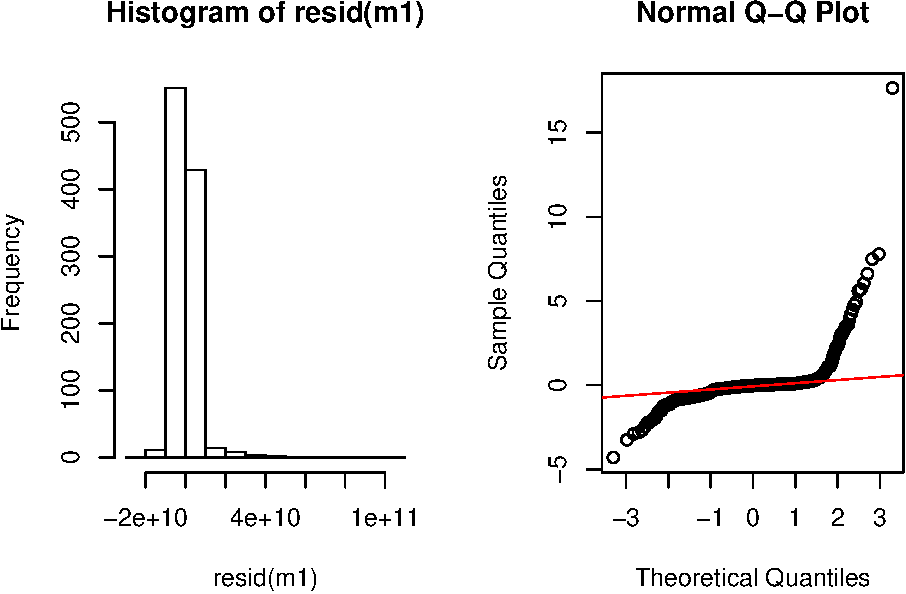
\includegraphics{report_files/figure-latex/unnamed-chunk-18-1.pdf}

It is clear that the residuals are not as normal as we like. The model
performs well for `typical' observations (between the -2 and 2
quartiles), but fails for the quite a few outlying observations. Both
positive and negative outliers have large residuals.

\begin{Shaded}
\begin{Highlighting}[]
\NormalTok{train_m1 <-}\StringTok{ }\NormalTok{train}
\NormalTok{train_m1}\OperatorTok{$}\NormalTok{resid <-}\StringTok{ }\KeywordTok{resid}\NormalTok{(m1)}
\NormalTok{train_m1 <-}\StringTok{ }\NormalTok{train_m1 }\OperatorTok\StringTok{ }
\StringTok{    }\KeywordTok{mutate}\NormalTok{(}\DataTypeTok{resid_abs =} \KeywordTok{abs}\NormalTok{(resid)) }\OperatorTok
\StringTok{    }\KeywordTok{arrange}\NormalTok{(}\KeywordTok{desc}\NormalTok{(resid))}
\KeywordTok{head}\NormalTok{(train_m1[}\KeywordTok{c}\NormalTok{(}\StringTok{'year'}\NormalTok{, }\StringTok{'country'}\NormalTok{, }\StringTok{'resid'}\NormalTok{)], }\DecValTok{10}\NormalTok{)}
\end{Highlighting}
\end{Shaded}

\begin{verbatim}
## # A tibble: 10 x 3
## # Groups:   country [4]
##     year country                resid
##    <int> <chr>                  <dbl>
##  1  2007 Netherlands    102855267532.
##  2  2009 Netherlands     45365348354.
##  3  2010 Luxembourg      43584466944.
##  4  2010 Netherlands     38522907898.
##  5  2006 Netherlands     35269523242.
##  6  2004 United Kingdom  33068662761.
##  7  2008 Netherlands     32645722874.
##  8  2010 United Kingdom  28689500402.
##  9  2008 Ireland         27763820382.
## 10  2004 Netherlands     26096392930.
\end{verbatim}

Interestingly, the top cases with the most errors are all developed
Western European allies of the U.S. \(M_1\) seems to have over-estimated
all of these cases, by tens of billions of dollars. Future work might
try to account for this by including an variable indicating if a country
is West European, or perhaps an (original) member of NATO.

Looking at the cases with negative residuals, the model seems to have
especially underestimated China and Japan, especially in the period
around the 2007--2008 years (during which there was an economic crisis).
My intuition is that some state of affairs---an overheated world market,
perhaps?---was directing excessive FDI to these countries over this time
period.

\hypertarget{m_2-linear-model-some-logged-variables}{%
\subsubsection{\texorpdfstring{\(M_2\): Linear Model, Some Logged
Variables}{M\_2: Linear Model, Some Logged Variables}}\label{m_2-linear-model-some-logged-variables}}

One way to make these residuals more normal is to log some of the poorly
behaved independent variables, transforming them to normality:

\begin{Shaded}
\begin{Highlighting}[]
\NormalTok{m2 <-}\StringTok{ }\KeywordTok{lm}\NormalTok{(fdi }\OperatorTok{~}\StringTok{ }\KeywordTok{log}\NormalTok{(population) }\OperatorTok{+}\StringTok{ }\NormalTok{arms_exports }\OperatorTok{+}\StringTok{ }\KeywordTok{as.factor}\NormalTok{(conflict) }\OperatorTok{+}\StringTok{ }
\StringTok{               }\KeywordTok{as.factor}\NormalTok{(alliance) }\OperatorTok{+}\StringTok{ }\NormalTok{km_dist }\OperatorTok{+}\StringTok{ }\KeywordTok{log}\NormalTok{(gdp) }\OperatorTok{+}\StringTok{ }\NormalTok{gdp_perc_growth }\OperatorTok{+}
\StringTok{               }\KeywordTok{as.factor}\NormalTok{(regime_type), train)}
\KeywordTok{summary}\NormalTok{(m2)}
\end{Highlighting}
\end{Shaded}

\begin{verbatim}
## 
## Call:
## lm(formula = fdi ~ log(population) + arms_exports + as.factor(conflict) + 
##     as.factor(alliance) + km_dist + log(gdp) + gdp_perc_growth + 
##     as.factor(regime_type), data = train)
## 
## Residuals:
##        Min         1Q     Median         3Q        Max 
## -2.592e+10 -1.482e+09 -3.372e+08  7.731e+08  1.021e+11 
## 
## Coefficients:
##                                           Estimate Std. Error t value
## (Intercept)                             -1.554e+10  2.807e+09  -5.539
## log(population)                         -2.219e+08  1.993e+08  -1.113
## arms_exports                             9.975e+05  1.291e+06   0.773
## as.factor(conflict)1                    -7.189e+08  5.897e+08  -1.219
## as.factor(alliance)1                     9.931e+08  5.511e+08   1.802
## km_dist                                 -3.895e+04  6.910e+04  -0.564
## log(gdp)                                 8.270e+08  1.622e+08   5.099
## gdp_perc_growth                         -1.550e+09  1.267e+09  -1.224
## as.factor(regime_type)closed anocracy    1.115e+09  7.054e+08   1.580
## as.factor(regime_type)conflict/occupied  7.597e+08  1.750e+09   0.434
## as.factor(regime_type)democracy          6.077e+07  6.125e+08   0.099
## as.factor(regime_type)full democracy     2.740e+09  7.337e+08   3.734
## as.factor(regime_type)open anocracy      6.930e+08  7.635e+08   0.908
##                                         Pr(>|t|)    
## (Intercept)                             3.89e-08 ***
## log(population)                         0.265983    
## arms_exports                            0.439887    
## as.factor(conflict)1                    0.223072    
## as.factor(alliance)1                    0.071812 .  
## km_dist                                 0.573041    
## log(gdp)                                4.08e-07 ***
## gdp_perc_growth                         0.221193    
## as.factor(regime_type)closed anocracy   0.114419    
## as.factor(regime_type)conflict/occupied 0.664196    
## as.factor(regime_type)democracy         0.920982    
## as.factor(regime_type)full democracy    0.000199 ***
## as.factor(regime_type)open anocracy     0.364291    
## ---
## Signif. codes:  0 '***' 0.001 '**' 0.01 '*' 0.05 '.' 0.1 ' ' 1
## 
## Residual standard error: 5.857e+09 on 1008 degrees of freedom
## Multiple R-squared:  0.1584, Adjusted R-squared:  0.1484 
## F-statistic: 15.82 on 12 and 1008 DF,  p-value: < 2.2e-16
\end{verbatim}

\begin{Shaded}
\begin{Highlighting}[]
\KeywordTok{mse}\NormalTok{(m2)}
\end{Highlighting}
\end{Shaded}

\begin{verbatim}
## [1] 3.386704e+19
\end{verbatim}

Logging these variables is actually slightly worse than \(M_1\), both in
terms of \(MSE\) and \(R^2\). In terms of variable significance, the
only change is that alliance becomes significant at \(p = .10\).
Residuals are almost identical to previous model.

\hypertarget{m_4-mixed-effects-panel-model}{%
\subsubsection{\texorpdfstring{\(M_4\): Mixed Effects Panel
Model}{M\_4: Mixed Effects Panel Model}}\label{m_4-mixed-effects-panel-model}}

This model attempts to deal with the fact that most subjects (states)
are sampled from multiple times. This kind of \emph{mixed effects}
models adds a second layer of \emph{random} effects to the usual
regression model's \emph{fixed} effects. This model will include country
as a variable in an attempt to quantify specific differences due to a
country that are not attributable to the independent variables.

\begin{Shaded}
\begin{Highlighting}[]
\NormalTok{m4 <-}\StringTok{ }\KeywordTok{lmer}\NormalTok{(fdi }\OperatorTok{~}\StringTok{ }\NormalTok{population }\OperatorTok{+}\StringTok{ }\NormalTok{arms_exports }\OperatorTok{+}\StringTok{ }\KeywordTok{as.factor}\NormalTok{(conflict) }\OperatorTok{+}\StringTok{ }
\StringTok{                 }\KeywordTok{as.factor}\NormalTok{(alliance) }\OperatorTok{+}\StringTok{ }\NormalTok{km_dist }\OperatorTok{+}\StringTok{ }\NormalTok{gdp }\OperatorTok{+}\StringTok{ }\NormalTok{gdp_perc_growth }\OperatorTok{+}
\StringTok{                 }\KeywordTok{as.factor}\NormalTok{(regime_type) }\OperatorTok{+}\StringTok{ }\NormalTok{(}\DecValTok{1} \OperatorTok{|}\StringTok{ }\NormalTok{country), train)}
\end{Highlighting}
\end{Shaded}

\begin{verbatim}
## Warning: Some predictor variables are on very different scales: consider
## rescaling
\end{verbatim}

\begin{Shaded}
\begin{Highlighting}[]
\KeywordTok{summary}\NormalTok{(m4)}
\end{Highlighting}
\end{Shaded}

\begin{verbatim}
## Linear mixed model fit by REML ['lmerMod']
## Formula: 
## fdi ~ population + arms_exports + as.factor(conflict) + as.factor(alliance) +  
##     km_dist + gdp + gdp_perc_growth + as.factor(regime_type) +  
##     (1 | country)
##    Data: train
## 
## REML criterion at convergence: 48034
## 
## Scaled residuals: 
##      Min       1Q   Median       3Q      Max 
## -13.1700  -0.0780  -0.0103   0.0418  16.6464 
## 
## Random effects:
##  Groups   Name        Variance  Std.Dev. 
##  country  (Intercept) 1.595e+19 3.993e+09
##  Residual             1.837e+19 4.285e+09
## Number of obs: 1021, groups:  country, 154
## 
## Fixed effects:
##                                           Estimate Std. Error t value
## (Intercept)                              8.819e+08  1.505e+09   0.586
## population                               7.535e-01  2.735e+00   0.276
## arms_exports                             2.863e+06  1.357e+06   2.109
## as.factor(conflict)1                    -5.032e+08  6.691e+08  -0.752
## as.factor(alliance)1                     9.608e+08  1.022e+09   0.940
## km_dist                                 -7.679e+04  1.276e+05  -0.602
## gdp                                      1.515e-03  5.745e-04   2.636
## gdp_perc_growth                         -1.213e+09  9.812e+08  -1.236
## as.factor(regime_type)closed anocracy    2.189e+08  1.027e+09   0.213
## as.factor(regime_type)conflict/occupied  1.260e+08  2.480e+09   0.051
## as.factor(regime_type)democracy          2.548e+07  9.524e+08   0.027
## as.factor(regime_type)full democracy     3.106e+09  1.198e+09   2.592
## as.factor(regime_type)open anocracy      8.678e+06  1.041e+09   0.008
\end{verbatim}

\begin{verbatim}
## 
## Correlation matrix not shown by default, as p = 13 > 12.
## Use print(x, correlation=TRUE)  or
##     vcov(x)        if you need it
\end{verbatim}

\begin{verbatim}
## fit warnings:
## Some predictor variables are on very different scales: consider rescaling
\end{verbatim}

\begin{Shaded}
\begin{Highlighting}[]
\KeywordTok{mse}\NormalTok{(m4)}
\end{Highlighting}
\end{Shaded}

\begin{verbatim}
## [1] 1.590054e+19
\end{verbatim}

From the \(MSE\) output, we see this model surpasses all previous
models. While it has 60 percent less error than the dummy model, this is
still a disappointing result.

However, with this model, \texttt{arms\_exports} becomes significant at
\(p = 0.05\)! GDP and full democracy also retain strongly significant
effects.

The residual plots are also more encouraging, as many of the extreme
errors we saw in \(M_1\) disappear. The theoretical quartile plot shows
a much nicer distribution, with less of a deviation from normality:

\begin{Shaded}
\begin{Highlighting}[]
\KeywordTok{par}\NormalTok{(}\DataTypeTok{mfrow=}\KeywordTok{c}\NormalTok{(}\DecValTok{1}\NormalTok{,}\DecValTok{2}\NormalTok{))}
\KeywordTok{hist}\NormalTok{(}\KeywordTok{resid}\NormalTok{(m4))}
\KeywordTok{qqnorm}\NormalTok{(}\KeywordTok{scale}\NormalTok{(}\KeywordTok{resid}\NormalTok{(m4))); }\KeywordTok{qqline}\NormalTok{(}\KeywordTok{scale}\NormalTok{(}\KeywordTok{resid}\NormalTok{(m4)), }\DataTypeTok{col=}\StringTok{'2'}\NormalTok{)}
\end{Highlighting}
\end{Shaded}

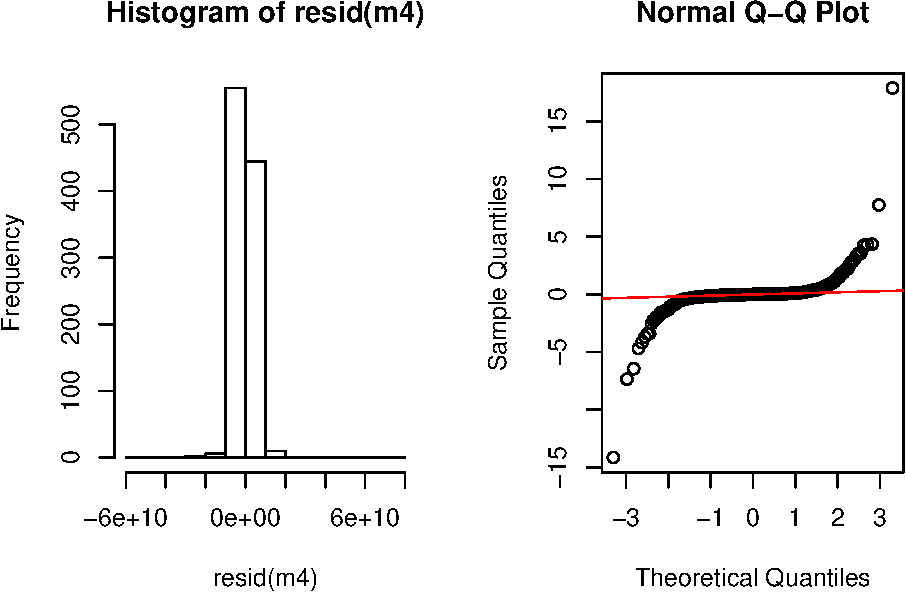
\includegraphics{report_files/figure-latex/unnamed-chunk-22-1.pdf}

Examining some of the largest residuals:

\begin{Shaded}
\begin{Highlighting}[]
\NormalTok{train_m4 <-}\StringTok{ }\NormalTok{train}
\NormalTok{train_m4}\OperatorTok{$}\NormalTok{resid <-}\StringTok{ }\KeywordTok{resid}\NormalTok{(m4)}
\NormalTok{train_m4 <-}\StringTok{ }\NormalTok{train_m4 }\OperatorTok\StringTok{ }
\StringTok{    }\KeywordTok{mutate}\NormalTok{(}\DataTypeTok{resid_abs =} \KeywordTok{abs}\NormalTok{(resid)) }\OperatorTok
\StringTok{    }\KeywordTok{arrange}\NormalTok{(}\KeywordTok{desc}\NormalTok{(resid))}
\KeywordTok{head}\NormalTok{(train_m4[}\KeywordTok{c}\NormalTok{(}\StringTok{'year'}\NormalTok{, }\StringTok{'country'}\NormalTok{)], }\DecValTok{10}\NormalTok{)}
\end{Highlighting}
\end{Shaded}

\begin{verbatim}
## # A tibble: 10 x 2
## # Groups:   country [7]
##     year country       
##    <int> <chr>         
##  1  2007 Netherlands   
##  2  2010 Luxembourg    
##  3  2008 Ireland       
##  4  2004 United Kingdom
##  5  2008 Switzerland   
##  6  2009 Netherlands   
##  7  2010 Ireland       
##  8  2010 United Kingdom
##  9  2010 Australia     
## 10  2004 Canada
\end{verbatim}

Like \(M_1\), the Netherlands and the U.K. are present, but appear less
often. Other countries include Ireland, Australia, and Canada. Again,
this suggests we might want to add a variable for either NATO or
English-speaking countries.

\hypertarget{m_5-mixed-effects-nato}{%
\subsubsection{\texorpdfstring{\(M_5\): Mixed Effects +
NATO}{M\_5: Mixed Effects + NATO}}\label{m_5-mixed-effects-nato}}

Since it's relatively simple, let's create a dummy variable indicating
whether a country was a founding member of NATO:

\begin{Shaded}
\begin{Highlighting}[]
\NormalTok{nato <-}\StringTok{ }\KeywordTok{c}\NormalTok{(}\StringTok{'Belgium'}\NormalTok{, }\StringTok{'Canada'}\NormalTok{, }\StringTok{'Denmark'}\NormalTok{, }\StringTok{'France'}\NormalTok{, }\StringTok{'Iceland'}\NormalTok{, }\StringTok{'Italy'}\NormalTok{,}
          \StringTok{'Luxembourg'}\NormalTok{, }\StringTok{'Netherlands'}\NormalTok{, }\StringTok{'Norway'}\NormalTok{, }\StringTok{'Portugal'}\NormalTok{,}
          \StringTok{'United Kingdom'}\NormalTok{, }\StringTok{'United States'}\NormalTok{)}

\NormalTok{train_m5 <-}\StringTok{ }\NormalTok{train }\OperatorTok
\StringTok{    }\KeywordTok{mutate}\NormalTok{(}\DataTypeTok{nato=}\KeywordTok{ifelse}\NormalTok{(country }\OperatorTok\StringTok{ }\NormalTok{nato, }\DecValTok{1}\NormalTok{, }\DecValTok{0}\NormalTok{))}

\NormalTok{m5 <-}\StringTok{ }\KeywordTok{lmer}\NormalTok{(fdi }\OperatorTok{~}\StringTok{ }\NormalTok{population }\OperatorTok{+}\StringTok{ }\NormalTok{arms_exports }\OperatorTok{+}\StringTok{ }\KeywordTok{as.factor}\NormalTok{(conflict) }\OperatorTok{+}\StringTok{ }
\StringTok{                 }\KeywordTok{as.factor}\NormalTok{(alliance) }\OperatorTok{+}\StringTok{ }\NormalTok{km_dist }\OperatorTok{+}\StringTok{ }\NormalTok{gdp }\OperatorTok{+}\StringTok{ }\NormalTok{gdp_perc_growth }\OperatorTok{+}
\StringTok{                 }\KeywordTok{as.factor}\NormalTok{(regime_type) }\OperatorTok{+}\StringTok{ }\KeywordTok{as.factor}\NormalTok{(nato) }\OperatorTok{+}\StringTok{  }\NormalTok{(}\DecValTok{1} \OperatorTok{|}\StringTok{ }\NormalTok{country),}
           \DataTypeTok{data=}\NormalTok{train_m5)}
\end{Highlighting}
\end{Shaded}

\begin{verbatim}
## Warning: Some predictor variables are on very different scales: consider
## rescaling
\end{verbatim}

\begin{Shaded}
\begin{Highlighting}[]
\KeywordTok{summary}\NormalTok{(m5)}
\end{Highlighting}
\end{Shaded}

\begin{verbatim}
## Linear mixed model fit by REML ['lmerMod']
## Formula: 
## fdi ~ population + arms_exports + as.factor(conflict) + as.factor(alliance) +  
##     km_dist + gdp + gdp_perc_growth + as.factor(regime_type) +  
##     as.factor(nato) + (1 | country)
##    Data: train_m5
## 
## REML criterion at convergence: 47956.5
## 
## Scaled residuals: 
##      Min       1Q   Median       3Q      Max 
## -13.1715  -0.0696  -0.0105   0.0396  16.6870 
## 
## Random effects:
##  Groups   Name        Variance  Std.Dev. 
##  country  (Intercept) 1.246e+19 3.530e+09
##  Residual             1.831e+19 4.279e+09
## Number of obs: 1021, groups:  country, 154
## 
## Fixed effects:
##                                           Estimate Std. Error t value
## (Intercept)                              6.414e+08  1.370e+09   0.468
## population                               1.521e+00  2.487e+00   0.612
## arms_exports                             3.092e+06  1.327e+06   2.329
## as.factor(conflict)1                    -4.185e+08  6.473e+08  -0.647
## as.factor(alliance)1                    -3.494e+08  9.502e+08  -0.368
## km_dist                                 -4.897e+04  1.155e+05  -0.424
## gdp                                      1.077e-03  5.429e-04   1.983
## gdp_perc_growth                         -1.233e+09  9.773e+08  -1.262
## as.factor(regime_type)closed anocracy    2.901e+08  9.638e+08   0.301
## as.factor(regime_type)conflict/occupied  8.905e+07  2.332e+09   0.038
## as.factor(regime_type)democracy          1.818e+08  8.886e+08   0.205
## as.factor(regime_type)full democracy     1.891e+09  1.125e+09   1.682
## as.factor(regime_type)open anocracy      1.828e+08  9.831e+08   0.186
## as.factor(nato)1                         9.033e+09  1.488e+09   6.071
\end{verbatim}

\begin{verbatim}
## 
## Correlation matrix not shown by default, as p = 14 > 12.
## Use print(x, correlation=TRUE)  or
##     vcov(x)        if you need it
\end{verbatim}

\begin{verbatim}
## fit warnings:
## Some predictor variables are on very different scales: consider rescaling
\end{verbatim}

\begin{Shaded}
\begin{Highlighting}[]
\KeywordTok{mse}\NormalTok{(m5)}
\end{Highlighting}
\end{Shaded}

\begin{verbatim}
## [1] 1.594544e+19
\end{verbatim}

Adding \texttt{nato} is very consequential to the model. Our main
independent variable \texttt{arms\_exports} becomes stronger and more
significant (\(p < .05\)). GDP becomes less significant, though it is
still significant at \(p < 0.05\). Population becomes more signficiant
but is `less important.' The full democracy indicator, becomes
insignicant at .05 and the magnitude of its coefficient decreases.

Interestingly, \(MSE\) is a smidge higher than \(M_4\), by 0.2 percent.
The residual graphs appear mostly the same as those of \(M_4\),
unfortunately.

\hypertarget{model-evaluations}{%
\section{Model Evaluations}\label{model-evaluations}}

We can now test our five models: \(M_0, M_1, M_2, M_4,\) and \(M_5\).
Reload the test data and get their predictions for the \texttt{test}
set:

\begin{Shaded}
\begin{Highlighting}[]
\NormalTok{test <-}\StringTok{ }\KeywordTok{read.csv}\NormalTok{(}\StringTok{'../data/clean/test.tsv'}\NormalTok{, }\DataTypeTok{sep=}\StringTok{'}\CharTok{\textbackslash{}t}\StringTok{'}\NormalTok{, }
                 \DataTypeTok{stringsAsFactors=}\OtherTok{FALSE}\NormalTok{)}

\NormalTok{test_m0 <-}\StringTok{ }\NormalTok{test }\OperatorTok\StringTok{ }
\StringTok{    }\KeywordTok{mutate}\NormalTok{(}\DataTypeTok{pred =} \KeywordTok{predict}\NormalTok{(m0, test),}
           \DataTypeTok{resid =}\NormalTok{ fdi }\OperatorTok{-}\StringTok{ }\NormalTok{pred)}
\NormalTok{test_m1 <-}\StringTok{ }\NormalTok{test }\OperatorTok\StringTok{ }
\StringTok{    }\KeywordTok{mutate}\NormalTok{(}\DataTypeTok{pred =} \KeywordTok{predict}\NormalTok{(m1, test),}
           \DataTypeTok{resid =}\NormalTok{ fdi }\OperatorTok{-}\StringTok{ }\NormalTok{pred)}
\NormalTok{test_m2 <-}\StringTok{ }\NormalTok{test }\OperatorTok\StringTok{ }
\StringTok{    }\KeywordTok{mutate}\NormalTok{(}\DataTypeTok{pred =} \KeywordTok{predict}\NormalTok{(m2, test),}
           \DataTypeTok{resid =}\NormalTok{ fdi }\OperatorTok{-}\StringTok{ }\NormalTok{pred)}
\NormalTok{test_m4 <-}\StringTok{ }\NormalTok{test }\OperatorTok\StringTok{ }
\StringTok{    }\KeywordTok{mutate}\NormalTok{(}\DataTypeTok{pred =} \KeywordTok{predict}\NormalTok{(m4, test),}
           \DataTypeTok{resid =}\NormalTok{ fdi }\OperatorTok{-}\StringTok{ }\NormalTok{pred)}

\CommentTok{# add NATO variable in}
\NormalTok{test_m5 <-}\StringTok{ }\NormalTok{test }\OperatorTok
\StringTok{    }\KeywordTok{mutate}\NormalTok{(}\DataTypeTok{nato=}\KeywordTok{ifelse}\NormalTok{(country }\OperatorTok\StringTok{ }\NormalTok{nato, }\DecValTok{1}\NormalTok{, }\DecValTok{0}\NormalTok{))}
\NormalTok{test_m5}\OperatorTok{$}\NormalTok{pred <-}\StringTok{ }\KeywordTok{predict}\NormalTok{(m5, test_m5)}
\NormalTok{test_m5}\OperatorTok{$}\NormalTok{resid <-}\StringTok{ }\NormalTok{test_m5}\OperatorTok{$}\NormalTok{fdi }\OperatorTok{-}\StringTok{ }\NormalTok{test_m5}\OperatorTok{$}\NormalTok{pred}
\end{Highlighting}
\end{Shaded}

Calculate \(MSE\) for each (divided by \(10^18\) for readability), in
order of best to worst:

\begin{Shaded}
\begin{Highlighting}[]
\KeywordTok{paste}\NormalTok{(}\StringTok{'M_5:'}\NormalTok{, }\KeywordTok{mean}\NormalTok{(test_m5}\OperatorTok{$}\NormalTok{resid}\OperatorTok{^}\DecValTok{2}\NormalTok{) }\OperatorTok{/}\StringTok{ }\DecValTok{10}\OperatorTok{^}\DecValTok{18}\NormalTok{)}
\end{Highlighting}
\end{Shaded}

\begin{verbatim}
## [1] "M_5: 18.3317314308561"
\end{verbatim}

\begin{Shaded}
\begin{Highlighting}[]
\KeywordTok{paste}\NormalTok{(}\StringTok{'M_4:'}\NormalTok{, }\KeywordTok{mean}\NormalTok{(test_m4}\OperatorTok{$}\NormalTok{resid}\OperatorTok{^}\DecValTok{2}\NormalTok{) }\OperatorTok{/}\StringTok{ }\DecValTok{10}\OperatorTok{^}\DecValTok{18}\NormalTok{)}
\end{Highlighting}
\end{Shaded}

\begin{verbatim}
## [1] "M_4: 18.7364181449195"
\end{verbatim}

\begin{Shaded}
\begin{Highlighting}[]
\KeywordTok{paste}\NormalTok{(}\StringTok{'M_2:'}\NormalTok{, }\KeywordTok{mean}\NormalTok{(test_m2}\OperatorTok{$}\NormalTok{resid}\OperatorTok{^}\DecValTok{2}\NormalTok{) }\OperatorTok{/}\StringTok{ }\DecValTok{10}\OperatorTok{^}\DecValTok{18}\NormalTok{)}
\end{Highlighting}
\end{Shaded}

\begin{verbatim}
## [1] "M_2: 51.6602441882049"
\end{verbatim}

\begin{Shaded}
\begin{Highlighting}[]
\KeywordTok{paste}\NormalTok{(}\StringTok{'M_1:'}\NormalTok{, }\KeywordTok{mean}\NormalTok{(test_m1}\OperatorTok{$}\NormalTok{resid}\OperatorTok{^}\DecValTok{2}\NormalTok{) }\OperatorTok{/}\StringTok{ }\DecValTok{10}\OperatorTok{^}\DecValTok{18}\NormalTok{)}
\end{Highlighting}
\end{Shaded}

\begin{verbatim}
## [1] "M_1: 53.8012662506875"
\end{verbatim}

\begin{Shaded}
\begin{Highlighting}[]
\KeywordTok{paste}\NormalTok{(}\StringTok{'M_0:'}\NormalTok{, }\KeywordTok{mean}\NormalTok{(test_m0}\OperatorTok{$}\NormalTok{resid}\OperatorTok{^}\DecValTok{2}\NormalTok{) }\OperatorTok{/}\StringTok{ }\DecValTok{10}\OperatorTok{^}\DecValTok{18}\NormalTok{)}
\end{Highlighting}
\end{Shaded}

\begin{verbatim}
## [1] "M_0: 63.9952822690553"
\end{verbatim}

Immediately it is clear that the mixed models, \(M_4\) and \(M_5\), have
far superior performance over the `vanilla' \(M_1\) and \(M_2\) (with
logged variables). Interesting, even though adding the \texttt{nato}
varible slightly decreased in-sample \(MSE\), it improved the model on
the test set.

Calculate \(R^2\), from best to worst:

\begin{Shaded}
\begin{Highlighting}[]
\KeywordTok{paste}\NormalTok{(}\StringTok{'M_5:'}\NormalTok{, }\KeywordTok{calc_r2}\NormalTok{(test_m5}\OperatorTok{$}\NormalTok{fdi, test_m5}\OperatorTok{$}\NormalTok{pred))}
\end{Highlighting}
\end{Shaded}

\begin{verbatim}
## [1] "M_5: 0.712975771040528"
\end{verbatim}

\begin{Shaded}
\begin{Highlighting}[]
\KeywordTok{paste}\NormalTok{(}\StringTok{'M_4:'}\NormalTok{, }\KeywordTok{calc_r2}\NormalTok{(test_m4}\OperatorTok{$}\NormalTok{fdi, test_m4}\OperatorTok{$}\NormalTok{pred))}
\end{Highlighting}
\end{Shaded}

\begin{verbatim}
## [1] "M_4: 0.706469257997731"
\end{verbatim}

\begin{Shaded}
\begin{Highlighting}[]
\KeywordTok{paste}\NormalTok{(}\StringTok{'M_2:'}\NormalTok{, }\KeywordTok{calc_r2}\NormalTok{(test_m2}\OperatorTok{$}\NormalTok{fdi, test_m2}\OperatorTok{$}\NormalTok{pred))}
\end{Highlighting}
\end{Shaded}

\begin{verbatim}
## [1] "M_2: 0.188953574659956"
\end{verbatim}

\begin{Shaded}
\begin{Highlighting}[]
\KeywordTok{paste}\NormalTok{(}\StringTok{'M_1:'}\NormalTok{, }\KeywordTok{calc_r2}\NormalTok{(test_m1}\OperatorTok{$}\NormalTok{fdi, test_m1}\OperatorTok{$}\NormalTok{pred))}
\end{Highlighting}
\end{Shaded}

\begin{verbatim}
## [1] "M_1: 0.156506262254786"
\end{verbatim}

\begin{Shaded}
\begin{Highlighting}[]
\KeywordTok{paste}\NormalTok{(}\StringTok{'M_0:'}\NormalTok{, }\KeywordTok{calc_r2}\NormalTok{(test_m0}\OperatorTok{$}\NormalTok{fdi, test_m0}\OperatorTok{$}\NormalTok{pred))}
\end{Highlighting}
\end{Shaded}

\begin{verbatim}
## [1] "M_0: 0"
\end{verbatim}

The ordering is the same as in the case of \(MSE\). I am pleased to see
the best model explains 71 percent of the variable in FDI! (Interesting,
the in-sample \(R^2\) for \(M_5\) is only .60.)

One final look at residuals, \(M_5\) on the test sample:

\begin{Shaded}
\begin{Highlighting}[]
\KeywordTok{par}\NormalTok{(}\DataTypeTok{mfrow=}\KeywordTok{c}\NormalTok{(}\DecValTok{1}\NormalTok{,}\DecValTok{2}\NormalTok{))}
\KeywordTok{hist}\NormalTok{(test_m5}\OperatorTok{$}\NormalTok{resid)}
\KeywordTok{qqnorm}\NormalTok{(}\KeywordTok{scale}\NormalTok{(test_m5}\OperatorTok{$}\NormalTok{resid)); }\KeywordTok{qqline}\NormalTok{(}\KeywordTok{scale}\NormalTok{(test_m5}\OperatorTok{$}\NormalTok{resid), }\DataTypeTok{col=}\StringTok{'2'}\NormalTok{)}
\end{Highlighting}
\end{Shaded}

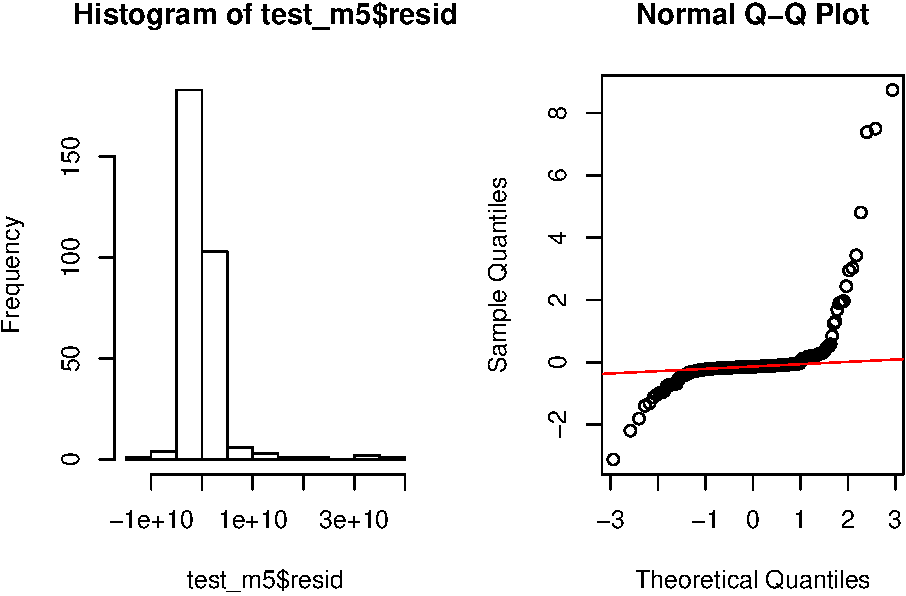
\includegraphics{report_files/figure-latex/unnamed-chunk-28-1.pdf}

The residuals histogram appears about the same shape as that of the
training set. However, the theoretical quartile plot is not as
smooth---their are many observations where predicted value is very far
from their actual value:

\begin{Shaded}
\begin{Highlighting}[]
\NormalTok{test_m5 <-}\StringTok{ }\KeywordTok{arrange}\NormalTok{(test_m5, }\KeywordTok{desc}\NormalTok{(resid))}
\KeywordTok{head}\NormalTok{(test_m5[}\KeywordTok{c}\NormalTok{(}\StringTok{'year'}\NormalTok{, }\StringTok{'country'}\NormalTok{, }\StringTok{'resid'}\NormalTok{)], }\DecValTok{10}\NormalTok{)}
\end{Highlighting}
\end{Shaded}

\begin{verbatim}
##    year        country       resid
## 1  2011    Netherlands 37699414141
## 2  2011     Luxembourg 32406834743
## 3  2011         Canada 31936016110
## 4  2012 United Kingdom 20971748405
## 5  2012     Luxembourg 15131703741
## 6  2012      Australia 13388939978
## 7  2012    Netherlands 13053412619
## 8  2012         Canada 10909575647
## 9  2012        Ireland  8886915986
## 10 2012    Switzerland  8734211652
\end{verbatim}

Among the largest residuals are the same old culprites: Netherlands, the
U.K., etc.

\hypertarget{conclusion}{%
\section{Conclusion}\label{conclusion}}

This paper confirmed the relationship between U.S. arms sales and U.S.
FDI. The more arms a country recieves from the U.S. in year \(t\), the
more direct foreign investment the country will recieve from the U.S.
the next year \(t+1\). This relationship is statistically significant,
even when controlling for other well-known factors influencing FDI.

I tested a number of models and found that mixed effect models best
capture the data set. The final model \(M_5\) performed the best,
explaining 71 percent of variation in \texttt{fdi} on the test dataset.

Other significant predictors of FDI include GDP and NATO membership,
which both have a positive effect (\(p < .05\)). Regime type of full
democracy also have a positive relationship with FDI at a lower
significance (\(p < .10\)).

Future work should focus on finding an explanation for why every
substantial model tended to overestimated FDI in a handful of highly
developed NATO allies, especially the Netherlands and the U.K.
Introducing the NATO membership as a variable helped, but was
insufficient to fully account for it.

\hypertarget{references}{%
\section{References}\label{references}}

Biglaiser, Glen, and Karl DeRouen, Jr. ``Following the Flag: Troop
Deployment and U.S. Foreign Direct Investment.'' \emph{International
Studies Quarterly} 51 (4): 835-854.

Center for Systemic Peace. 2017. \emph{Polity IV Annual Time-Series,
1800-2017} (Excel file).
\textless{}\url{http://www.systemicpeace.org/inscrdata.html}\textgreater{}.

Gibler, Douglas M. 2013. ``Formal Alliances (v4.1).''
\emph{International Military Alliances, 1648-2008}. CQ Press.
\textless{}\url{http://www.correlatesofwar.org/data-sets/formal-alliances}\textgreater{}.

Gilpin, Robert. 1987. \emph{The Political Economy of International
Relations}. Princeton: Princeton University Press.

Gleditsch, Kristian Skrede. \_Distance Between Capital Cities."
\textless{}\url{http://ksgleditsch.com/data-5.html}\textgreater{}.

Gleditsch, Nils Petter, Peter Wallensteen, Mikael Eriksson, Margareta
Sollenberg, and Håvard Strand. 2002. ``Armed Conflict 1946-2001: A New
Dataset.'' \emph{Journal of Peace Research} 39 (5).

Gowa, Joanne. 1994. \emph{Allies, Adversaries, and International Trade}.
Princeton: Princeton University Press.

Gowa, Joanne, and Edward D. Mansfield. 1993. ``Power Politics and
International Trade.'' \emph{American Political Science Review} 87 (2):
408-20.

Little, Andrea, and David Leblang. 2004. ``Military Securities:
Financial Flows and the Deployment of U.S. Troops.'' In \emph{Annual
Meeting of the American Political Science Association}. Chicago, IL.

Long, Andrew G. 2003. ``Defense Pacts and International Trade.''
\emph{Journal of Peace Research} 40 (5): 537--52.

OECD. 2018. ``Benchmark definition, 3rd edition (BMD3): Foreign direct
investment: flows by partner country.'' \emph{OECD International Direct
Investment Statistics} (database).

Rugman, Alan M., and Alain Verbeke. 2001. ``Location, Competitiveness,
and the Multinational Enterprise.'' In \emph{Oxford Handbook of
International Business}, ed. A. M. Rugman and T. L. Brewer. Oxford:
Oxford University Press.

Stockholm International Peace Research Institute. \emph{Arms Transfers
Database}.
\textless{}\url{https://www.sipri.org/databases/armstransfers}\textgreater{}.

World Bank. 2018. \emph{National Accounts Data}.
\textless{}\url{https://data.worldbank.org/indicator/NY.GDP.MKTP.CD}\textgreater{}.

United Nations, Population Division. ``Total Population - Both Sexes''
(Excel file).
\textless{}\url{https://population.un.org/wpp/Download/Standard/Population/}\textgreater{}.


\end{document}
